\subsection{Experimental Setup}
\label{sec:setup}

We use a server that has two $16$-core x86-based Intel Xeon Gold 6226R processors running at $2.90$ GHz. Each core has an L1 cache of $1$ MB, an L2 cache of $16$ MB, and a shared L3 cache of $22$ MB. The machine has $93.4$ GB of system memory and runs on CentOS Stream 8. We use GCC 8.5 and OpenMP 4.5. Table \ref{tab:dataset} shows the graphs we use in our experiments. All of them are obtained from the SuiteSparse Matrix Collection \cite{suite19}.

\begin{table}[hbtp]
  \centering
  \caption{List of $13$ graphs obtained SuiteSparse Matrix Collection \cite{suite19} (directed graphs are marked with $*$). Here, $|V|$ is the number of vertices, $|E|$ is the number of edges (after adding reverse edges), $D_{avg}$ is the average degree, and $|\Gamma|$ is the number of communities obtained using LPA.\ignore{In the table, B refers to a billion, M refers to a million and K refers a thousand.}}
  \label{tab:dataset}
  \begin{tabular}{|c||c|c|c|c|}
    \toprule
    \textbf{Graph} &
    \textbf{\textbf{$|V|$}} &
    \textbf{\textbf{$|E|$}} &
    \textbf{\textbf{$D_{avg}$}} &
    \textbf{\textbf{$|\Gamma|$}} \\
    % \textbf{$1 - \Gamma_G$} \\
    \midrule
    \multicolumn{5}{|c|}{\textbf{Web Graphs (LAW)}} \\ \hline
    indochina-2004$^*$ & 7.41M & 341M & 41.0 & 4.24K \\ \hline  % & \num{4.7e-4} & 2.9 GB
    uk-2002$^*$ & 18.5M & 567M & 16.1 & 42.8K \\ \hline  % & \num{9.6e-5} & 16 GB
    arabic-2005$^*$ & 22.7M & 1.21B & 28.2 & 3.66K \\ \hline  % & \num{5.5e-4} & 11 GB
    uk-2005$^*$ & 39.5M & 1.73B & 23.7 & 20.8K \\ \hline  % & \num{9.6e-5} & 16 GB
    webbase-2001$^*$ & 118M & 1.89B & 8.6 & 2.76M \\ \hline  % & \num{7.3e-7} & 18 GB
    it-2004$^*$ & 41.3M & 2.19B & 27.9 & 5.28K \\ \hline  % & \num{3.8e-4} & 19 GB
    sk-2005$^*$ & 50.6M & 3.80B & 38.5 & 3.47K \\ \hline  % & \num{5.8e-4} & 33 GB
    \multicolumn{5}{|c|}{\textbf{Social Networks (SNAP)}} \\ \hline
    com-LiveJournal & 4.00M & 69.4M & 17.4 & 2.54K \\ \hline  % & \num{7.9e-4} & 480 MB
    com-Orkut & 3.07M & 234M & 76.2 & 29 \\ \hline  % & \num{6.7e-2} & 1.7 GB
    \multicolumn{5}{|c|}{\textbf{Road Networks (DIMACS10)}} \\ \hline
    asia\_osm & 12.0M & 25.4M & 2.1 & 2.38K \\ \hline  % & \num{8.4e-4} & 200 MB
    europe\_osm & 50.9M & 108M & 2.1 & 3.05K \\ \hline  % & \num{6.6e-4} & 910 MB
    \multicolumn{5}{|c|}{\textbf{Protein k-mer Graphs (GenBank)}} \\ \hline
    kmer\_A2a & 171M & 361M & 2.1 & 21.2K \\ \hline  % & \num{9.4e-5} & 3.2 GB
    kmer\_V1r & 214M & 465M & 2.2 & 6.17K \\ \hline  % & \num{3.2e-4} & 4.2 GB
  \bottomrule
  \end{tabular}
\end{table}
% We convert directed graphs (marked with $*$) to undirected by duplicating edges in the reverse direction, and set the weight of each edge to $1$. and $F_{size}$ is size of the \textit{MatrixMarket} file

\begin{figure*}[hbtp]
  \centering
  \subfigure[Runtime in seconds (logarithmic scale) with \textit{FLPA}, \textit{igraph LPA}, \textit{NetworKit LPA}, and \textit{GVE-LPA}]{
    \label{fig:rak-compare--runtime}
    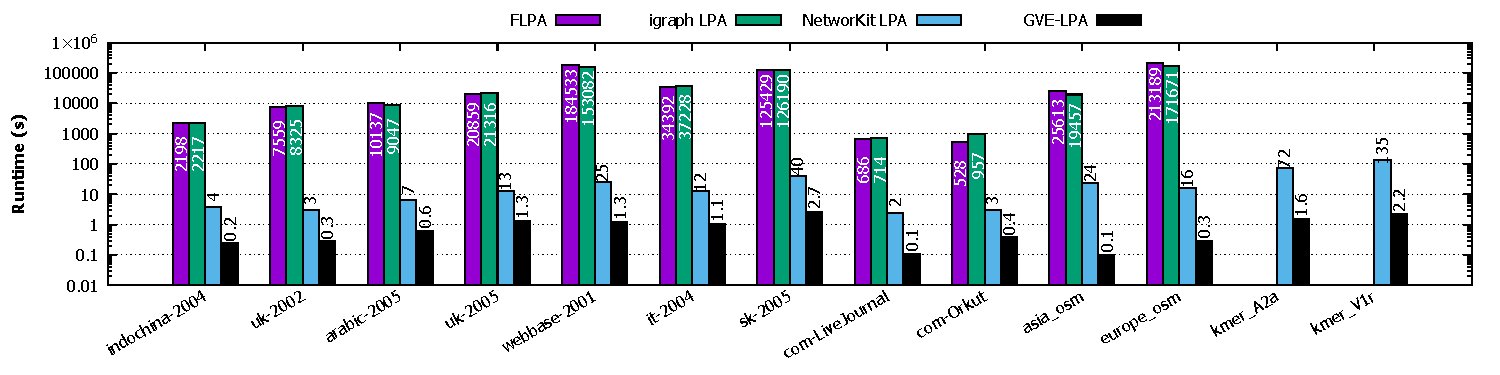
\includegraphics[width=0.98\linewidth]{out/rak-runtime.pdf}
  } \\[-0ex]
  \subfigure[Speedup (logarithmic scale) of \textit{GVE-LPA} with respect to \textit{FLPA}, \textit{igraph LPA}, \textit{NetworKit LPA}.]{
    \label{fig:rak-compare--speedup}
    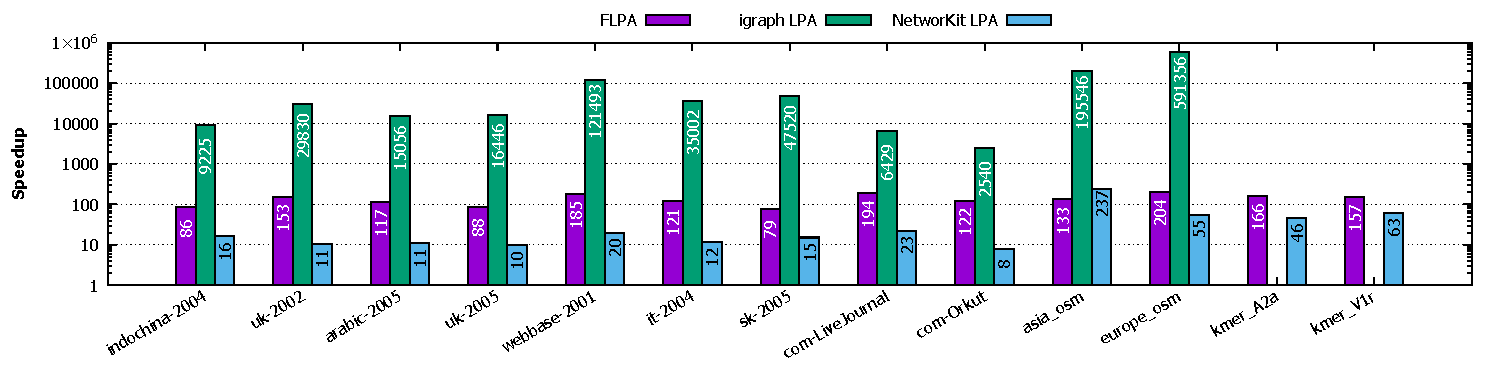
\includegraphics[width=0.98\linewidth]{out/rak-speedup.pdf}
  } \\[-0ex]
  \subfigure[Modularity of communities obtained with \textit{FLPA}, \textit{igraph LPA}, \textit{NetworKit LPA}, and \textit{GVE-LPA}.]{
    \label{fig:rak-compare--modularity}
    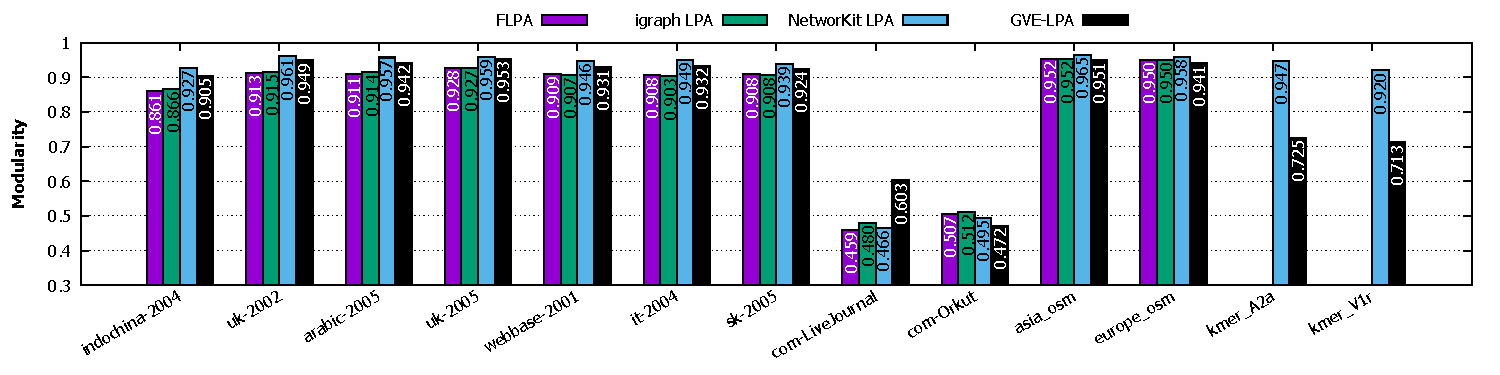
\includegraphics[width=0.98\linewidth]{out/rak-modularity.pdf}
  } \\[-2ex]
  \caption{Runtime\ignore{in seconds (logarithmic scale)}, speedup, and modularity of communities obtained with \textit{FLPA}, \textit{igraph LPA}, \textit{NetworKit LPA}, and \textit{GVE-LPA} for each graph\ignore{in the dataset}. \textit{FLPA} and \textit{igraph LPA} fail to run on \textit{kmer\_A2a} and \textit{kmer\_V1r} graphs, and thus their results are not shown.}
  \label{fig:rak-compare}
\end{figure*}





\subsection{Comparing Performance of GVE-LPA}

We now compare the performance of GVE-LPA with igraph LPA, FLPA, and NetworKit LPA. For Vite, we convert the graph datasets to Vite's binary graph format, run it on a single node\ignore{(Vite supports distributed community detection)} with threshold cycling/scaling optimization, and measure the reported average total time. For Grappolo, we measure the run it on the same system, and measure the reported total time. For NetworKit, we use a Python script to invoke \texttt{PLM} (Parallel Louvain Method), and measure the total time reported with \texttt{getTiming()}. For each graph, we measure the runtime of each implementation five times, for averaging. We also record the modularity of communities obtained, as reported by each implementation.

Figure \ref{fig:rak-compare--runtime} shows the runtimes of Vite (Louvain), Grappolo (Louvain), NetworKit Louvain, and GVE-Louvain on each graph in the dataset. Figure \ref{fig:rak-compare--speedup} shows the speedup of GVE-Louvain with respect to each implementation mentioned above. GVE-Louvain is on average $50\times$, $22\times$, and $20\times$ faster than Vite, Grappolo, and NetworKit respectively. On the \textit{sk-2005} graph, GVE-Louvain finds communities in $6.8$ seconds, and thus achieve a processing rate of $560$ million edges/s. Figure \ref{fig:rak-compare--modularity} shows the modularity of communities obtained with each implementation. GVE-Louvain on average obtains $3.1\%$ higher modularity than Vite (especially on web graphs), and $0.6\%$ lower modularity than Grappolo and NetworKit (especially on social networks with poor clustering).

\begin{figure}[hbtp]
  \centering
  \subfigure{
    \label{fig:rak-hardness--all}
    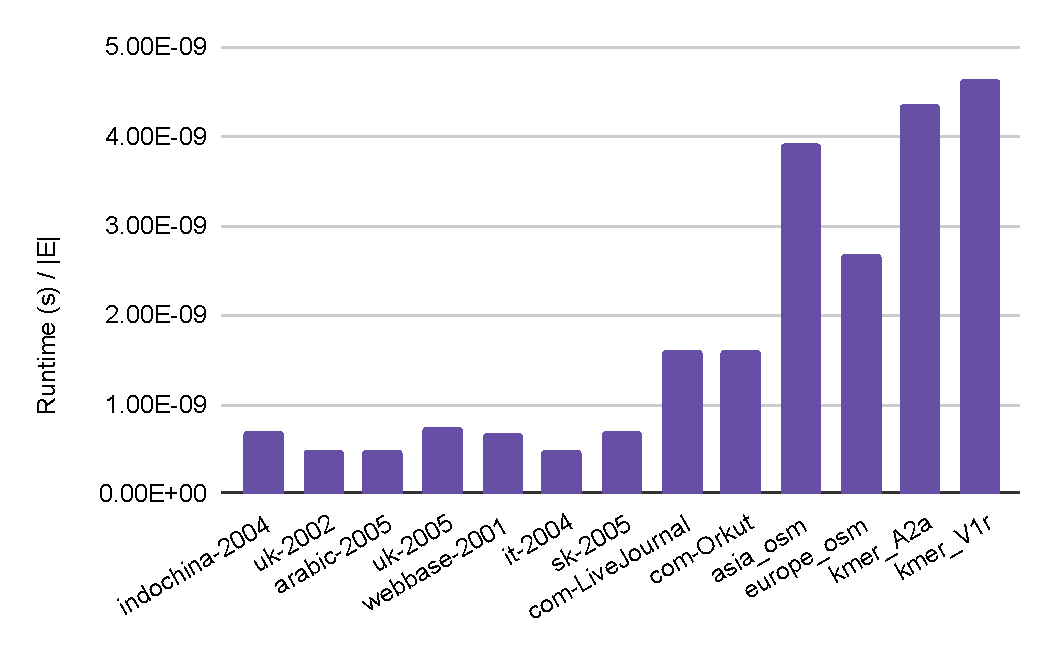
\includegraphics[width=0.98\linewidth]{out/rak-hardness.pdf}
  } \\[-2ex]
  \caption{Runtime $/ |E|$ factor with \textit{GVE-LPA} for each graph in the dataset.}
  \label{fig:rak-hardness}
\end{figure}

\begin{figure}[hbtp]
  \centering
  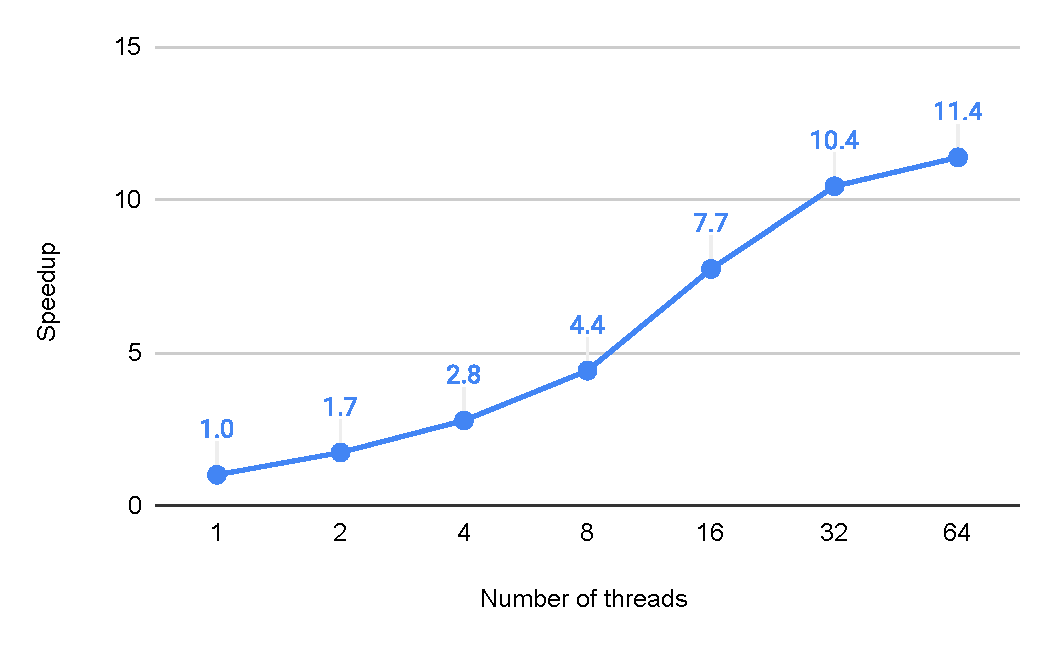
\includegraphics[width=0.98\linewidth]{out/rak-ss.pdf} \\[0ex]
  \caption{Average speedup of \textit{GVE-LPA} with increasing number of threads (in multiples of 2).}
  \label{fig:rak-ss}
\end{figure}





\subsection{Analyzing Performance of GVE-LPA}

The phase-wise and pass-wise split of GVE-Louvain is shown in Figures \ref{fig:louvain-splits--phase} and \ref{fig:louvain-splits--pass} respectively. Figure \ref{fig:louvain-splits--phase} indicates that GVE-Louvain spends most of the runtime in the local-moving phase on \textit{web graphs}, \textit{road networks}, and \textit{protein k-mer graphs}, while it devotes majority of the runtime in the aggregation phase on \textit{social networks}. The pass-wise split (Figure \ref{fig:louvain-splits--pass}) indicates that the first pass dominates runtime on high-degree graphs (\textit{web graphs} and \textit{social networks}), while subsequent passes prevail in execution time on low-degree graphs (\textit{road networks} and \textit{protein k-mer graphs}).

On average, $49\%$ of GVE-Louvain's runtime is spent in the local-moving phase, $35\%$ is spent in the aggregation phase, and $16\%$ is spent in other steps (initialization, renumbering communities, looking up dendrogram, and resetting communities) of the algorithm. Further, $67\%$ of the runtime is spent in the first pass of the algorithm, which is the most expensive pass due to the size of the original graph (later passes work on super-vertex graphs) \cite{com-wickramaarachchi14}.

We also observe that graphs with lower average degree (\textit{road networks} and \textit{protein k-mer graphs}) and graphs with poor community structure (such as \verb|com-LiveJournal| and \verb|com-Orkut|) have a larger $\text{runtime}/|E|$ factor, as shown in Figure \ref{fig:rak-hardness}.





\subsection{Strong Scaling of GVE-LPA}

Finally, we measure the strong scaling performance of GVE-Louvain. To this end, we adjust the number of threads from $1$ to $64$ in multiples of $2$ for each input graph, and measure the time taken for finding communities with GVE-Louvain (five times for averaging). The results are shown in Figure \ref{fig:rak-ss}. With 32 threads, GVE-Louvain obtains a $10.4\times$ speedup compared to running with a single thread, i.e., its performance increases by $1.6\times$ for every doubling of threads. Scaling is limited due to the various sequential steps/phases in the algorithm. At 64 threads, GVE-Louvain is impacted by NUMA effects, and offer speedups of only $11.4\times$.
